\documentclass[11pt]{article}
\usepackage{graphicx}
\usepackage[export]{adjustbox}
\usepackage{float}
\usepackage{amsmath}
\title{EE302 Homework 1}
\date{2018\\ March}
\author{Nail Tosun - 2094563 -Section 5\\ Electric and Electronic Engineering Departmant, METU}
\begin{document}
\maketitle
2)
	Since system is first order there is no overshoot. By solving the differential equation analytically;
	$$T(s)=\frac{\frac{4}{s+1}}{1+\frac{4}{s+1}}$$
	$$T(s)=\frac{4}{s+5}$$
	$$Y(s)=\frac{4}{s(s+5)}$$
	$$y(t) = \frac{4}{5}-\frac{4}{5}e^{-5t} \> \> t>0 $$
	$$\tau=\frac{1}{a}=0.2 sec$$ 
	$$T_s=4\tau=0.8 sec$$
	$$e(\infty)=1-0.8=0.2$$ 
	

\begin{figure}[H]
  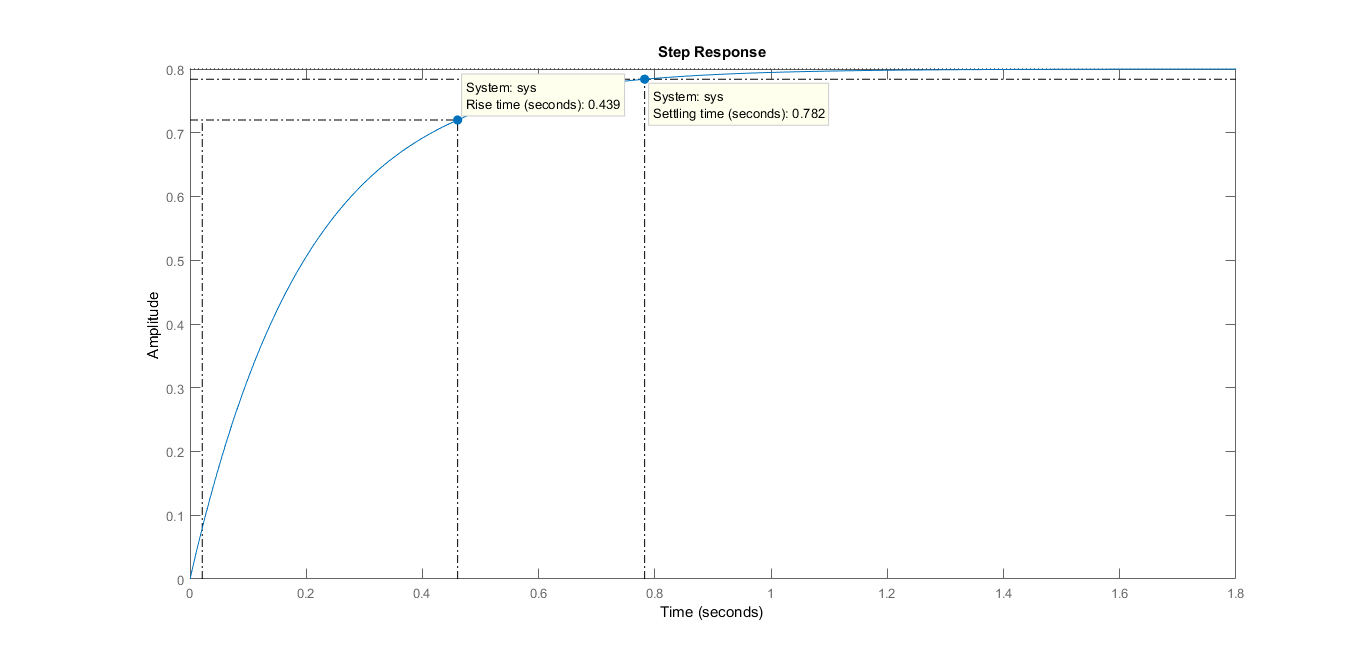
\includegraphics[scale=0.7, center]{step1}
  \caption{Step response of the system}
  \label{fig:zero}
\end{figure}
The results are as expected.

\[T(s)=\frac{\frac{20s+4}{5s(s+1)}}{1+\frac{20s+4}{5s(s+1)}}\]
\[T(s)=\frac{20s+4}{5s^2+25s+4}\]
\[Y(s)=\frac{20s+4}{s(5s^2+25s+4)}\]
System has 2 negative real pole and 1 negative real zero.
$$Pole_1=-4.83 \> Pole_2=-0.165 \> Zero=-0.2$$
Since one of the pole is so close to zero we can do pole-zero cancellation. Then we can solve like first order system.


\begin{figure}[H]
  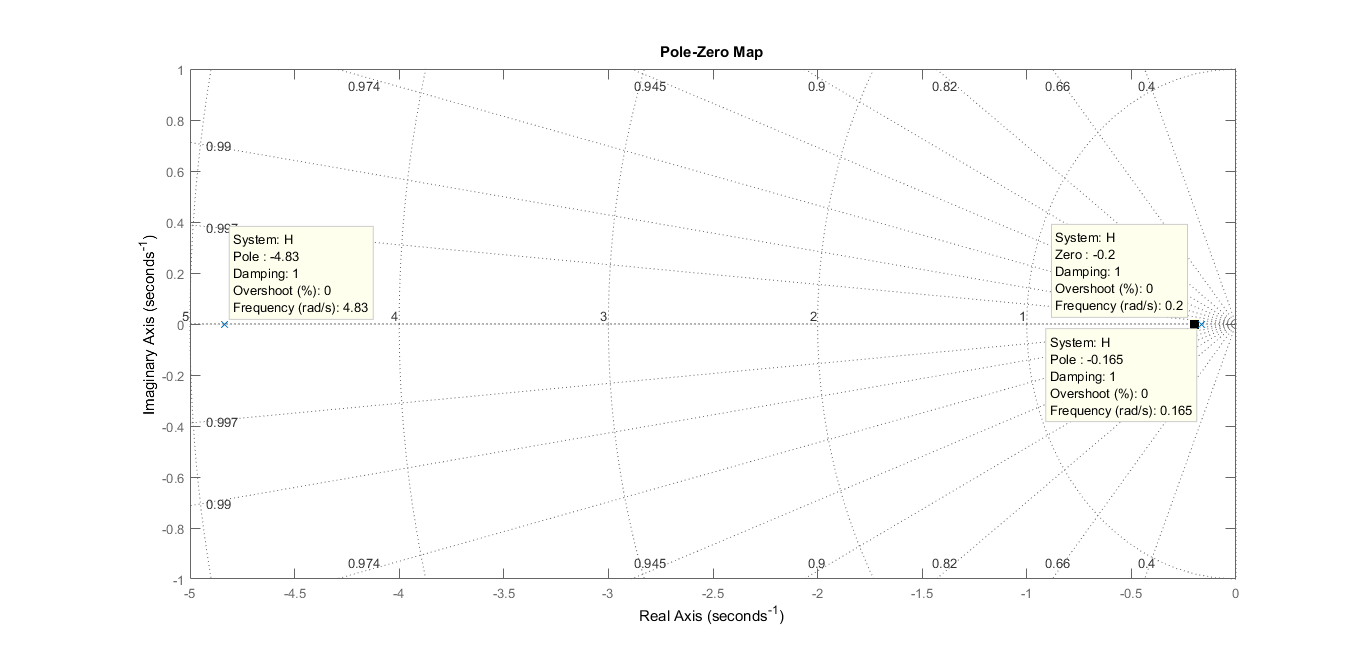
\includegraphics[scale=0.7, center]{polezero}
  \caption{Pole-zero diagram of the system}
  \label{fig:zero}
\end{figure}
\begin{figure}[H]
  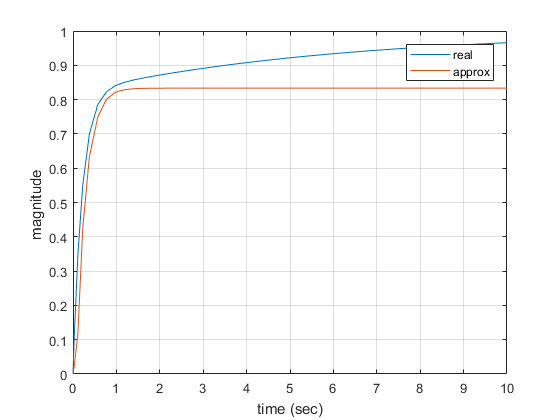
\includegraphics[scale=0.7, center]{approx}
  \caption{Step response of the system}
  \label{fig:zero}
\end{figure}
$$T(s)=\frac{1}{0.25+1}$$
$$y(t)=1-e^{-4t}$$
$$\tau=0.25 sec$$
$$t_{settle}=4\tau=1 sec$$
Since it is an overdamped system (before approximation) there is no overshoot.
$$t_{rise}=\frac{2}{a}=0.5 sec$$

\begin{figure}[H]
  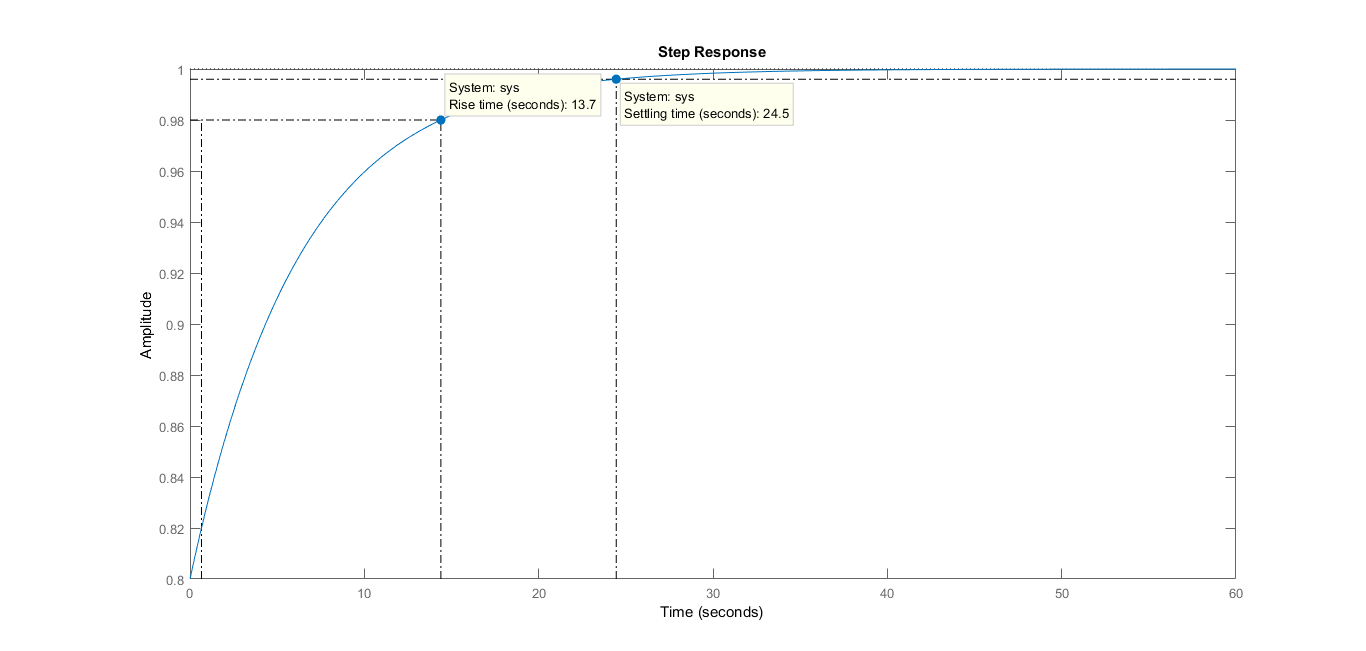
\includegraphics[scale=0.7, center]{step2}
  \caption{Step response of the system with PI controller where P=4 and I=0.8}
  \label{fig:zero}
\end{figure}

d)

\[D(s)=\frac{4s+10}{s}\]
\[G(s)=\frac{4s+10}{(s+1)}\]
\[T(s)=\frac{G(s)}{1+G(s)}\]
\[T(s)=\frac{4s+10}{s^2+5s+10}\]
\[Y(s)=\frac{4s+10}{s(s^2+5s+10)}\]
\[Y(s)=\frac{1}{s}+\frac{Bs+C}{s^2+5s+10}\]
\[Y(s)=\frac{1}{s}-\frac{s+1}{s^2+5s+10}\]
\[Y(s)=\frac{1}{s}-\frac{s+1}{(s+2.5)^2+3.75}\]
\[Y(s)=\frac{1}{s}-\frac{s+2.5}{(s+2.5)^2+3.75}-\frac{1.5}{(s+2.5)^2+3.75}\]
\[y(t)=1-e^{-\frac{5t}{2}}(cos(1.9t)-0.77sin(1.9t))\]



\begin{figure}[H]
  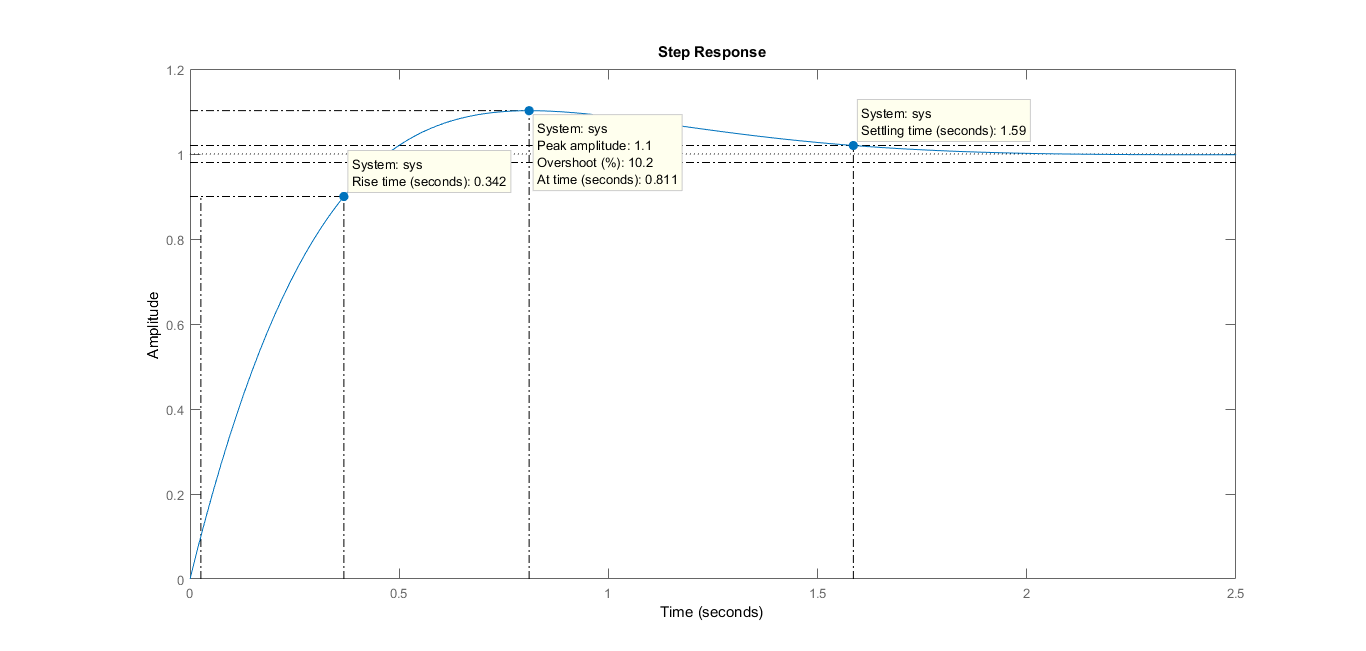
\includegraphics[scale=0.7, center]{step3}
  \caption{Step response of the system with PI controller P=4 I=10}
  \label{fig:zero}
\end{figure}


Without controller unit i have significant steady state error. Using PI controller help about this issue. When i used I=0.8 system is to slow to response. However when i increase I to 10 system response time significantly improved. (Settling time 24.5 sec to 1.59 sec). But with increasing I there is overshooting problem but trade-off is okey. 

3)

\[\frac{G(s)}{1+G(s)}=\frac{Ks+b}{s^2+as+b}\]
\[G(s)(s^2+(a-k)s)=Ks+b\]
\[G(s)=\frac{Ks+b}{s(s+a-k)}\]


b)

$$K_v=\frac{1}{\lim_{s\to 0} sG(s)}=0.04$$
\[\lim{s\to 0} \frac{s^2r+sm}{s^2+ns}=25 \> by L'hospital\] 
$$\frac{m}{n}=25$$
\[T(s)=\frac{G(s)}{1+G(s)}\]
\[T(s)=\frac{rs+m}{s^2+(n+r)s+m}\]
$$m=25$$
$$n=1$$
\[Y(s)=\frac{A}{s}+\frac{\delta(s+3)}{s^2+6s+25}+\frac{\beta5}{s^2+6s+25}\]
\[n+r=6\]
$$r=5$$

c)

\[T(s)=\frac{5s+25}{s^2+6s+25}\]
\[Y(s)=\frac{5s+25}{s(s^2+6s+25)}\]
\[T(s)=\frac{5s+15}{(s+3)^2+4^2}+\frac{10}{(s+3)^2+4^2}\]
\[25A=25\]
$$A=1$$
$$\delta=5$$
$$\beta=\frac{5}{8}$$

d)

$$M_p=e^{\frac{-\pi}{tan\phi}}$$
\[\omega_n=5 \> \omega_d=4\]
\[\phi=arctan(\frac{4}{3})\]
$$M_p=0.105$$

4)

\[T(s)=\frac{\frac{G(s)}{s}}{1+\frac{G(s)}{s}}\]
\[T(s)=\frac{4}{s^2+2s+4}\]
\[\omega_n=2\]
\[\omega_d=\sqrt{3}\]
\[tan(\phi)=\sqrt{3}\]
\[M_p=e^{-\frac{\pi}{tan(\phi)}}\]
\[M_p=0.163\]
\[e_{unit}=\lim_{s \to 0} G(s)\]
\[e_{unit}=\lim_{s \to 0} \frac{4}{s(s+2)}=0 \>\> Type1 \> system\]
\[e_{ramp}=\lim_{s \to 0} sG(s)=2\]

\[\lim_{s \to \inf} \frac{4K_i}{s+2}=8\]
$$K_i=4$$

\[T(s)=\frac{16}{s^2+2s+16}\]
\[tan(\phi)=\frac{\sqrt{15}}{1}\]
$$M_p=0.444$$
With increasing $K_i$ increases overshoot percentage.
\begin{figure}[H]
  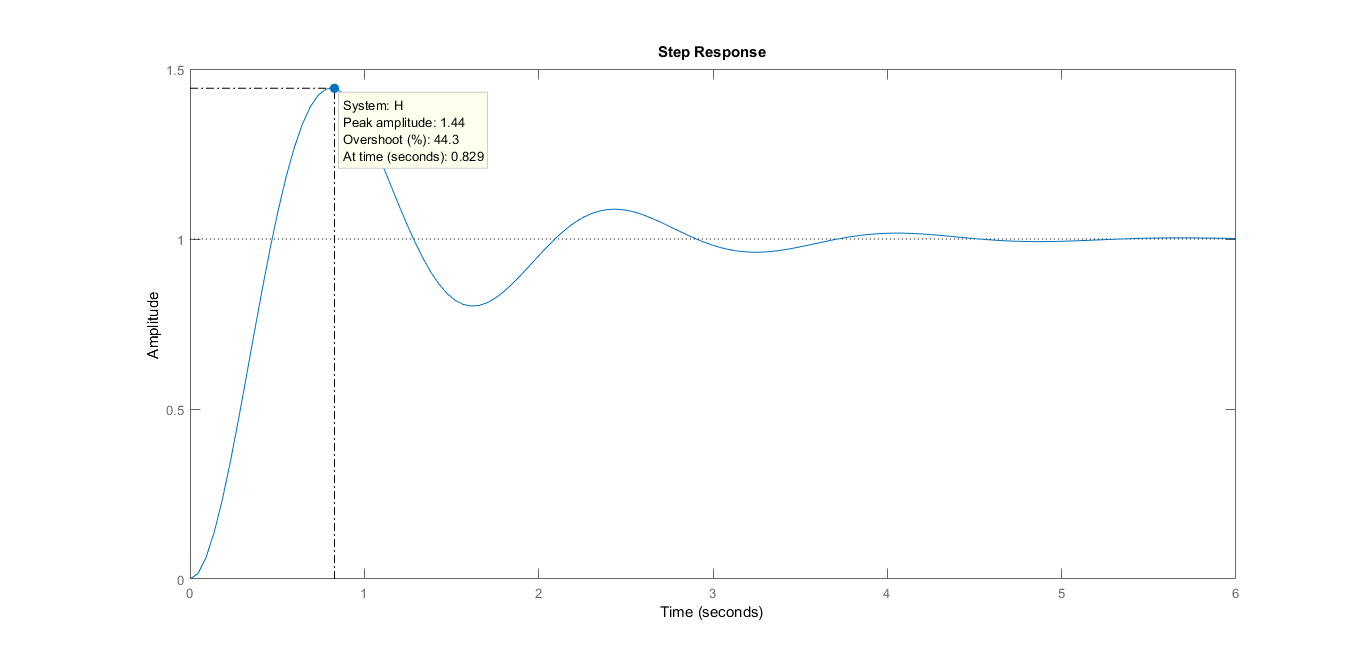
\includegraphics[scale=0.7, center]{mal}
  \caption{Step response $K_i=4$}
  \label{fig:zero}
\end{figure}  

5)

a)

\[A(s)=\frac{100(s+2)}{s^2-1}\]
\[(E(s)G_c(s)+D(s))A(s)=Y(s)\]
\[E(s)=R(s)-Y(s)\]
\[((R(s)-Y(s))G_c(s)+D(s))A(s)=Y(s)\]
\[R(s)G_c(s)A(s)+D(s)A(s)=Y(s)(1+G_c(s)A(s))\]
$$G_r(s)=\frac{G_c(s)A(s)}{1+G_c(s)A(s)}$$
$$G_d(s)=\frac{A(s)}{1+G_c(s)A(s)}$$

b)

\[C(s)=G_c(s)A(s)E(s)+D(s)A(s)\]
\[C(s)=R(s)-E(s)\]
\[E(s)=\frac{R(s)-D(s)A(s)}{1+A(s)G_c(s)} \> where \> G_c(s)=1 \> and \> R(s)=\frac{1}{s}\]
\[E(s)=\frac{\frac{1}{s}-\frac{100(s+2)}{s(s^2-1)}}{1+\frac{100(s+2)}{s^2-1}}\]
$$e_r(\infty)=\lim_{s\to 0} sE(s)$$
$$e_r(\infty)=\lim_{s\to 0} \frac{1-\frac{100(s+2)}{s^2-1}}{1+\frac{100(s+2)}{s^2-1}}=-\frac{199}{201}$$

c)
\[E(s)=\frac{\frac{1}{s}}{1+\frac{(s+\alpha)100(s+2)}{s(s^2-1)}}\]
$$e_r(\infty)=\lim_{s\to 0} sE(s)$$
$$e_r(\infty)=\lim_{s\to 0} \frac{1}{1+\frac{(s+\alpha)100(s+2)}{s(s^2-1)}}=0$$

d)
\begin{figure}[H]
  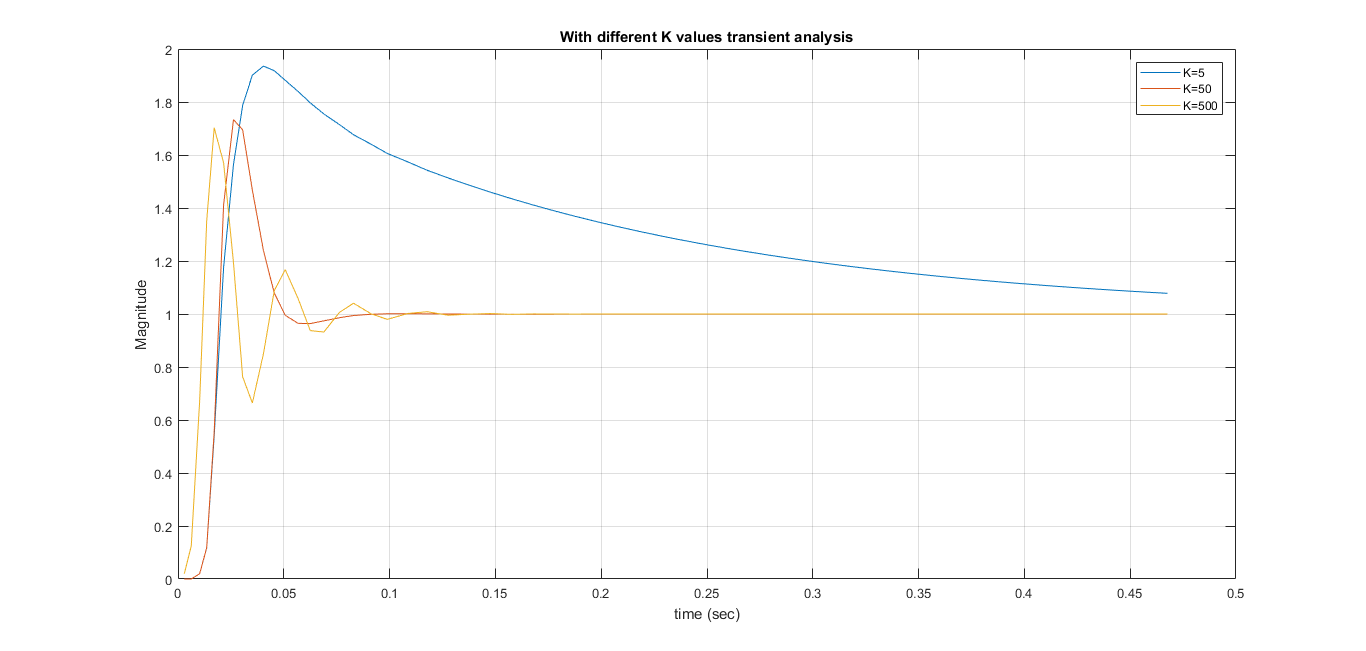
\includegraphics[scale=0.7, center]{differentk}
  \caption{Transient Analysis}
  \label{fig:zero}
\end{figure}
Increasing k means that we increased the integrator controller. With increasing integrator we have faster response means that shorter $t_{rise}$ and $t_{settling}$. However the trade-off is oscillation frequency increased. 

e)

\[E(s)=-\frac{\frac{100(s+2)}{s(s^2-1)}}{1+\frac{100(s+2)}{(s^2-1)}}\]
$$e_r(\infty)=\lim_{s\to 0} sE(s)$$
$$e_r(\infty)=\lim_{s\to 0} -\frac{\frac{100(s+2)}{s^2-1}}{1+\frac{100(s+2)}{s^2-1}}=\frac{200}{199}$$

\begin{figure}[H]
  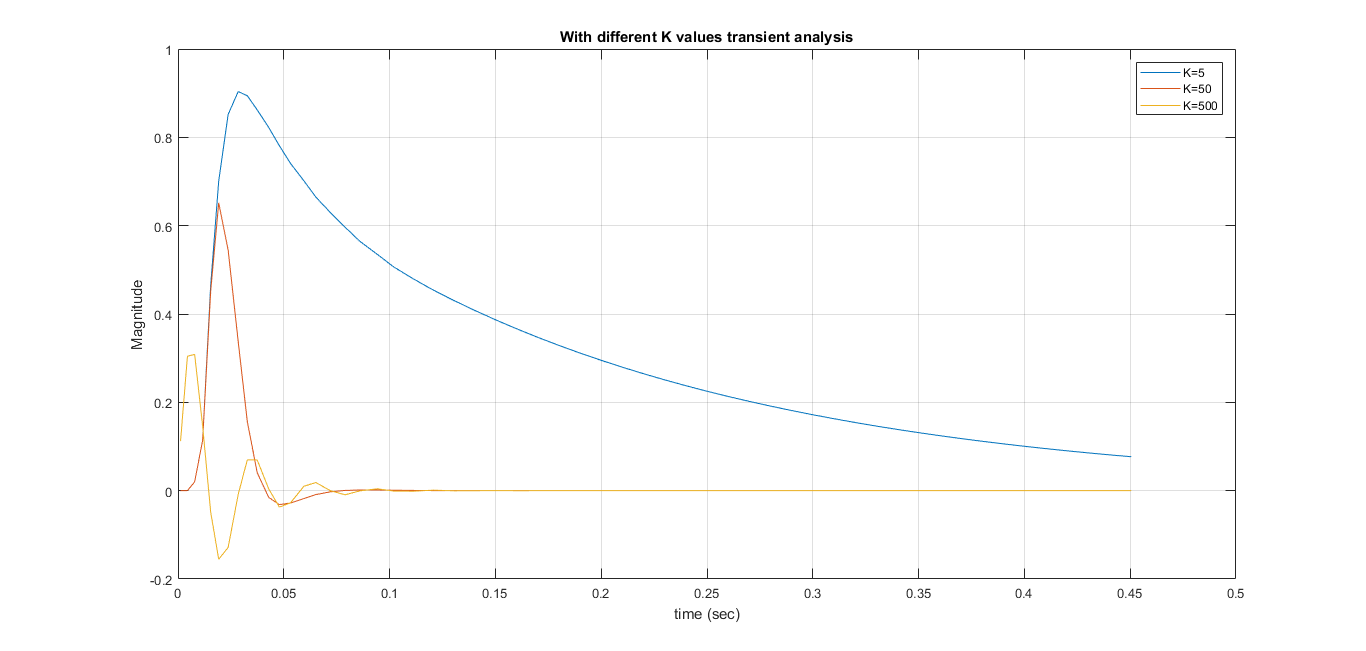
\includegraphics[scale=0.7, center]{differentk1}
  \caption{Transient Analysis}
  \label{fig:zero}
\end{figure}



\end{document}